\documentclass[tikz,border=6pt]{standalone}

\usepackage{amsmath}
\usepackage{pgfplots}
\usepgfplotslibrary{groupplots}
\pgfplotsset{compat=1.18}

%--------------------------------------------------
% Kiểu chung cho mỗi ô đồ thị
%--------------------------------------------------
\pgfplotsset{
  myaxis/.style={
    width=4.2cm,
    height=4.2cm,
    scale only axis,
    axis lines=middle,
    axis line style={black, line width=0.5pt},
    xtick=\empty,
    ytick=\empty,
    tick style={draw=none},
    xlabel={},
    ylabel={},
    enlargelimits=false,
    clip=true,
    samples=200,
    smooth,
    every axis plot/.append style={black, line width=1pt},
    after end axis/.code={
      \draw[line width=0.5pt] (rel axis cs:0,0) rectangle (rel axis cs:1,1);
    }
  }
}

\begin{document}

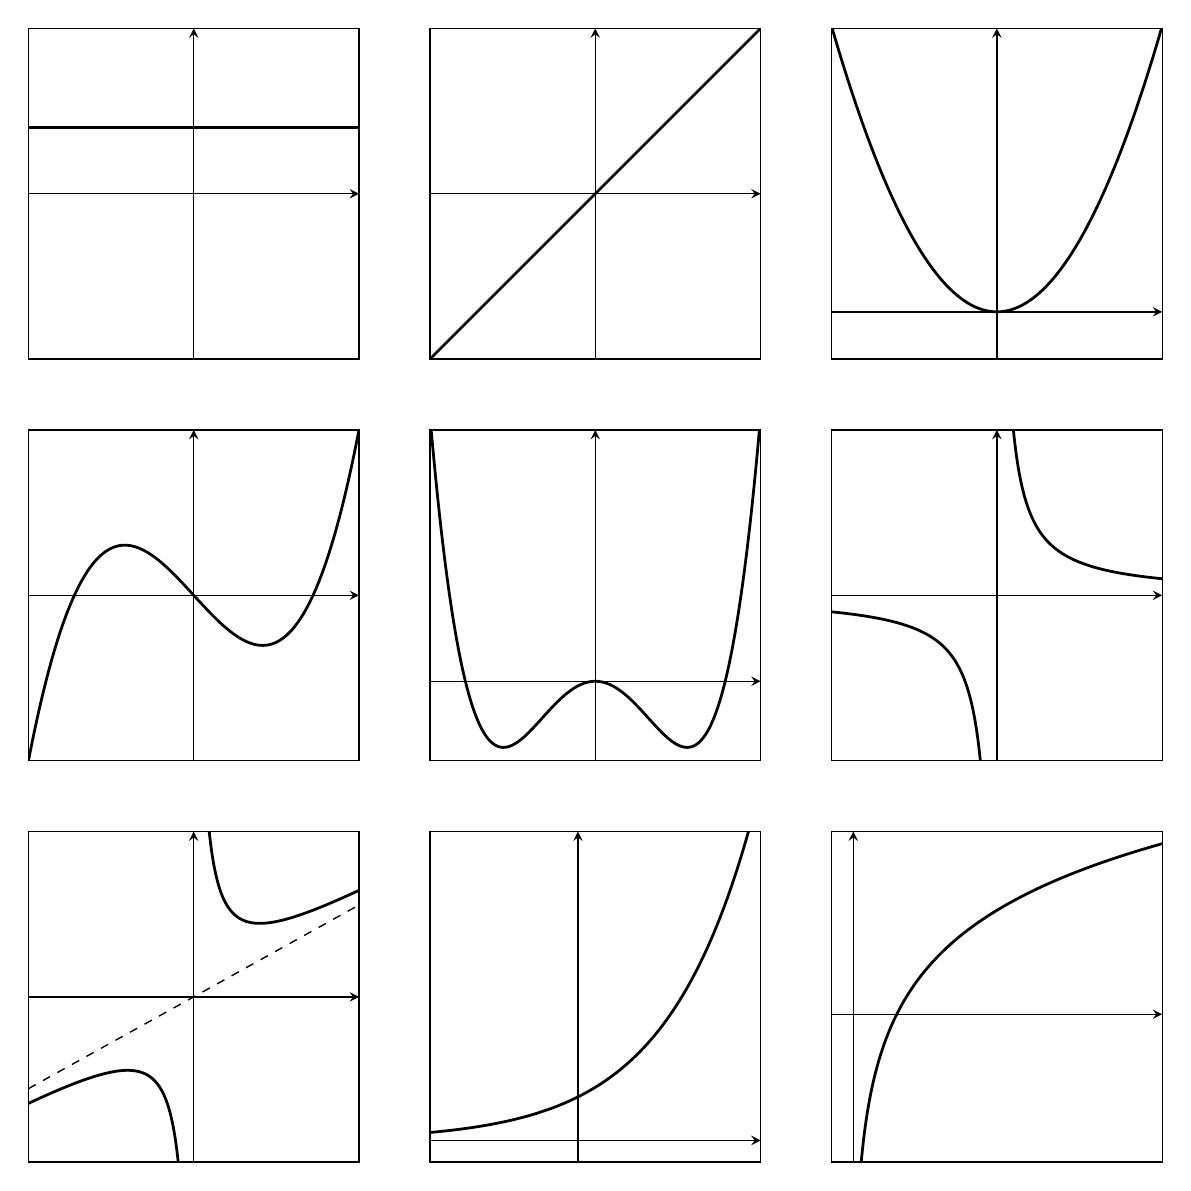
\begin{tikzpicture}
\begin{groupplot}[
  group style={
    group size=3 by 3,
    horizontal sep=0.9cm,
    vertical sep=0.9cm
  }
]

%==================================================
% Hàng 1
%==================================================

% 1) y = 1
\nextgroupplot[
  myaxis,
  xmin=-2.5, xmax=2.5,
  ymin=-2.5, ymax=2.5
]
\addplot[domain=-2.5:2.5] {1};

% 2) y = x
\nextgroupplot[
  myaxis,
  xmin=-2.5, xmax=2.5,
  ymin=-2.5, ymax=2.5
]
\addplot[domain=-2.5:2.5] {x};

% 3) y = x^2
\nextgroupplot[
  myaxis,
  xmin=-2.2, xmax=2.2,
  ymin=-0.8, ymax=4.8
]
\addplot[domain=-2.2:2.2] {x^2};

%==================================================
% Hàng 2
%==================================================

% 4) y = (1/3)x^3 - x
\nextgroupplot[
  myaxis,
  xmin=-2.4, xmax=2.4,
  ymin=-2.2, ymax=2.2
]
\addplot[domain=-2.4:2.4] {x^3/3 - x};

% 5) y = (1/4)x^4 - (1/2)x^2
\nextgroupplot[
  myaxis,
  xmin=-1.8, xmax=1.8,
  ymin=-0.3, ymax=.95
]
\addplot[domain=-2.2:2.2] {x^4/4 - x^2/2};

% 6) y = 1/x
\nextgroupplot[
  myaxis,
  xmin=-2.5, xmax=2.5,
  ymin=-4.0, ymax=4.0
]
\addplot[domain=-2.5:-0.2] {1/x};
\addplot[domain=0.2:2.5] {1/x};

%==================================================
% Hàng 3
%==================================================

% 7) y = x + 1/x
\nextgroupplot[
  myaxis,
  xmin=-2.5, xmax=2.5,
  ymin=-4.5, ymax=4.5
]
\addplot[domain=-2.5:-0.05] {x + 1/x};
\addplot[domain=0.05:2.5] {x + 1/x};
\addplot[domain=-2.5:2.5, dashed, line width=.5pt] {x};

% 8) y = exp(x)
\nextgroupplot[
  myaxis,
  xmin=-1.7, xmax=2.1,
  ymin=-0.5, ymax=7.1
]
\addplot[domain=-2.3:2.0] {exp(x)};

% 9) y = ln(x)
\nextgroupplot[
  myaxis,
  xmin=-0.5, xmax=7.1,
  ymin=-1.7, ymax=2.1
]
\addplot[domain=0.05:9.0] {ln(x)};

\end{groupplot}
\end{tikzpicture}

\end{document}